\documentclass[a0paper,portrait]{baposter}

%----------------------------------------------------------------------------------------
%	SIMPLE BOXED ENVIRONMENT
%----------------------------------------------------------------------------------------

\usepackage{wrapfig}
\usepackage{lmodern}

\usepackage[utf8]{inputenc} %unicode support
\usepackage[T1]{fontenc}
\usepackage{amsmath}

\selectcolormodel{cmyk}

\graphicspath{{figures/}} % Directory in which figures are stored


\newcommand{\compresslist}{%
\setlength{\itemsep}{0pt}%
\setlength{\parskip}{1pt}%
\setlength{\parsep}{0pt}%
}

\newenvironment{boenumerate}
  {\begin{enumerate}\renewcommand\labelenumi{\textbf\theenumi.}}
  {\end{enumerate}}

% kaobox (while tcolorbox may be more rich, I find it too complicated so I prefer mdframed)
\RequirePackage{tikz}
\RequirePackage[framemethod=TikZ]{mdframed}

%\mdfsetup{skipabove=\topskip,skipbelow=0pt}
\mdfdefinestyle{kaoboxstyle}{
	skipabove=1.5\topskip,
	skipbelow=.5\topskip,
	rightmargin=0pt,
	leftmargin=0pt,
	%innertopmargin=3pt,
	%innerbottommargin=3pt,
	innerrightmargin=7pt,
	innerleftmargin=7pt,
	topline=false,
	bottomline=false,
	rightline=false,
	leftline=false,
	%linewidth=1pt,
	%roundcorner=0pt,
	%font={},
	%frametitlefont={},
	frametitlerule=true,
	linecolor=black,
	%backgroundcolor=LightBlue,
	fontcolor=black,
	%frametitlebackgroundcolor=LightBlue,
}

\newmdenv[
	style=kaoboxstyle,
	backgroundcolor=lightgreen!25,
	frametitlebackgroundcolor=lightgreen!25,
]{kaobox}


\begin{document}


\definecolor{darkgreen}{cmyk}{0.8,0,0.8,0.45}
\definecolor{lightgreen}{cmyk}{0.8,0,0.8,0.25}

\begin{poster}
{
grid=false,
headerborder=open, % Adds a border around the header of content boxes
colspacing=1em, % Column spacing
bgColorOne=white, % Background color for the gradient on the left side of the poster
bgColorTwo=white, % Background color for the gradient on the right side of the poster
borderColor=darkgreen, % Border color
headerColorOne=lightgreen, % Background color for the header in the content boxes (left side)
headerColorTwo=lightgreen, % Background color for the header in the content boxes (right side)
headerFontColor=white, % Text color for the header text in the content boxes
boxColorOne=white, % Background color of the content boxes
textborder=rounded, %rectangle, % Format of the border around content boxes, can be: none, bars, coils, triangles, rectangle, rounded, roundedsmall, roundedright or faded
eyecatcher=false, % Set to false for ignoring the left logo in the title and move the title left
headerheight=0.11\textheight, % Height of the header
headershape=rounded, % Specify the rounded corner in the content box headers, can be: rectangle, small-rounded, roundedright, roundedleft or rounded
headershade=plain,
headerfont=\Large\textsf, % Large, bold and sans serif font in the headers of content boxes
%textfont={\setlength{\parindent}{1.5em}}, % Uncomment for paragraph indentation
linewidth=2pt % Width of the border lines around content boxes
}
{}
%
%----------------------------------------------------------------------------------------
%	TITLE AND AUTHOR NAME
%----------------------------------------------------------------------------------------
%
{
\textsf %Sans Serif
{Can a Nuclear Reactor be Anywhere?
}
} % Poster title
% {\vspace{1em} Marta Stepniewska, Pawel Siedlecki\\ % Author names
% {\small \vspace{0.7em} Department of Bioinformatics, Institute of Biochemistry and Biophysics, PAS, Warsaw, Pawinskiego 5a}} % Author email addresses
{\sf\vspace{0.5em}\\
A look into the challenges of finding appropriate sites for nuclear reactors and the factors in play.
}
{
\includegraphics[width=35mm,scale=0.35]{favpng_question-mark-logo-information}} % University/lab logo


\headerbox{1. Case Study}{name=introduction,column=0,row=0, span=3}{
Nuclear energy is an important part of the clean energy mix. It does not emit $\mathrm{CO_2}$ directly, though its construction and the mining of uranium cause low indirect emissions. While a clean energy, nuclear does come with drawbacks, from several angles: uranium supply, accident risk, radioactive waste, and proliferation concerns notably. In this factsheet we discuss the accident risk issue and how that relates to the siting of nuclear reactors.
}


\headerbox{2. Regulations and Economy}{name=model,column=0,below=introduction,span=1}{

Siting a nuclear power plant is a complex process. One needs to assess several physical characteristics, as well as societal ones.

\begin{itemize}\compresslist
\item Seismic Risk
\item Landslide Risk
\item Flooding Risk
\item Protected Areas
\item Population Density
\item Water Access
\item Infrastructure Access
\end{itemize}

We want to be in a low-risk zone in term of natural hazards, in a region where the construction is possible (infrastructure access and right to build), and relatively close to water. At the same time, we'd like to be close to population centers to allow for more efficient electricity transport, while respecting guidance on exclusion zones. A lot of these societal parameters can vary, depending on the risk tolerance at a given location and the type of reactor considered.


}


\headerbox{3. Energy Needs}{name=mcs,column=0,below=model,span=1}{
% https://econ.washington.edu/sites/econ/files/old-site-uploads/2014/06/Olsen-Wolff-2014-NuclearPaper.pdf
By taking high resolution satellite imagery of the Earth at Night, and combining this with high resolution population data, we can estimate the regions of the world in energy poverty. In red on the map below shown for Africa, the regions where energy is most needed, on top of transitioning the current generation sources to clean energy.

\begin{center}
    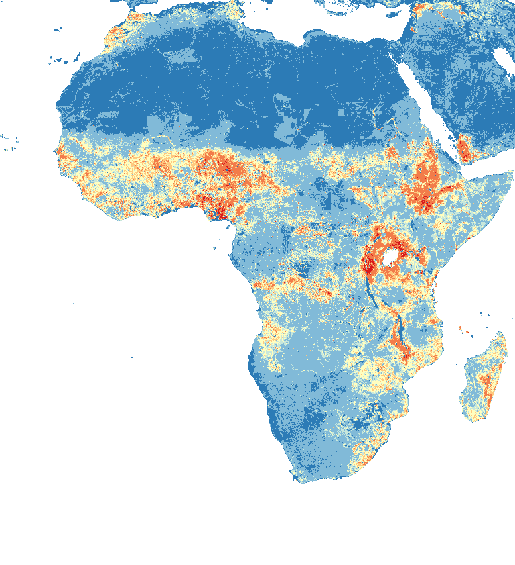
\includegraphics[width=100pt]{energy_poverty_01deg_3mwh_cf95_africa}
\end{center}



}

\headerbox{4. Nuclear Presence}{name=screen,span=2,column=1,below=introduction}{ % To reduce this block to 1 column width, remove 'span=2'

%Image attribution:
%https://www.irena.org/energytransition/Power-Sector-Transformation/Hydrogen-from-Renewable-Power

\begin{center}
    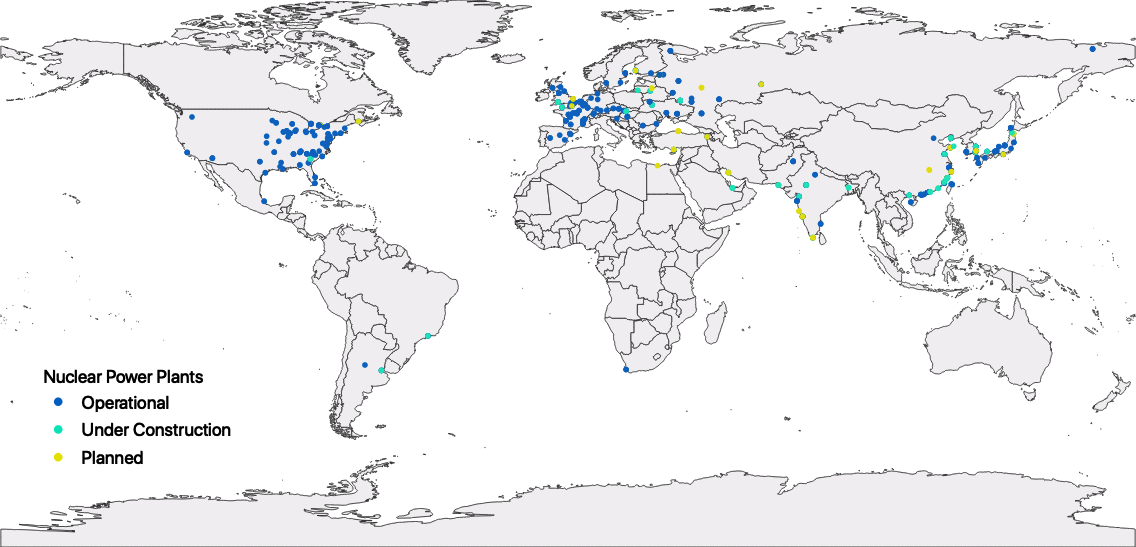
\includegraphics[width=\linewidth]{nuclear_plants_map}
\end{center}


}

\headerbox{5. Africa Siting Potential}{name=sea,span=2,column=1,below=screen}{ % To reduce this block to 1 column width, remove 'span=2'

%\begin{center}
%    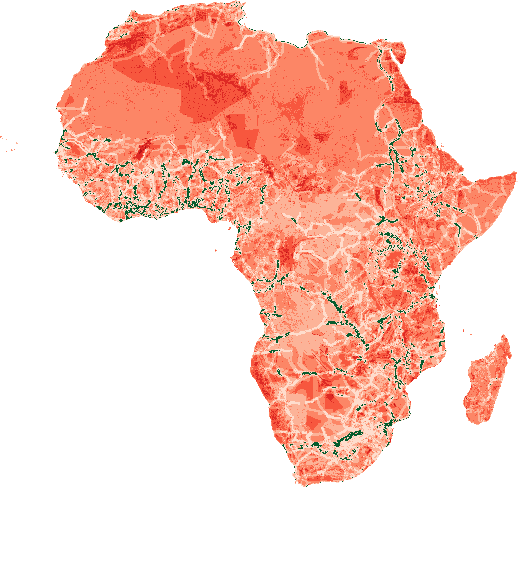
\includegraphics[width=\linewidth]{africa_siting}
%\end{center}
\begin{wrapfigure}{l}{0.5\textwidth}
    \begin{center}
        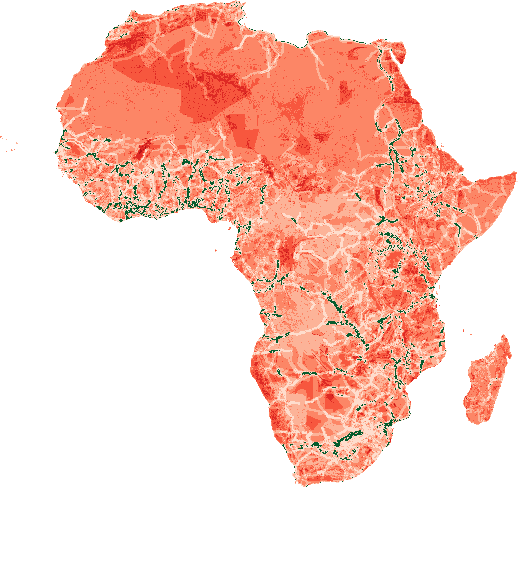
\includegraphics[width=\linewidth]{africa_siting}
    \end{center}
    %\vspace{-145pt}
\end{wrapfigure}


Let us apply our siting filters to Africa as an example. In this case, we used relatively high precision data (down to a kilometer) to assess the local population density, natural hazard exposure, distance to a sufficient water source, and other requirements. The various shades of red denote location where one or more filters are negative (the darker the red, the more issues the location present). A light red shading implies that only one filter eliminated the region. Depending on which one, this may be designed for and improve the chances to develop a stable grid. In green, we can see the optimal locations. The first thing that is striking is the amount of red shown. Most locations are not adequate, mostly due to two dominant factors: water access and existing infrastructure. Some countries show very little potential, notably Lybia (only part of the coast are available) due to an extreme lack of water resources. Finding ways to relax water requirements (smaller reactors, with a smaller water footprint) and the needs for existing infrastructure (transmission lines) would increase the locations and allow for an easier deployment of nuclear energy.




\begin{kaobox}[frametitle=Common Questions]
\begin{itemize}
\item \textit{What about proliferation?}

It has been shown that conflict risks, combined with access to nuclear technology, even civilian projects, had an impact on nations pursuing a nuclear weapon program. Note that this does not mean that they would have the means to do it in less than a decade. I personally would not recommend siting a nuclear reactor in, say, South Sudan at this time.

\end{itemize}
\end{kaobox}

}


\headerbox{6. Conclusions}{name=conclusion,column=1,below=sea,span=2,above=bottom}{
% DeCAF is a chemoinformatical tool that can be helpful in ligand-based drug design.
% It provides a comprehensive molecule description and a fast algorithms for comparing and aligning multiple ligands.
\begin{boenumerate}\compresslist
    \item Nuclear is a dense energy. A small land area can consequently power a large region. However, the cost of developing infrastructure in developing countries can be extremely large.
    \item Some region could benefit from a nuclear reactor. A lot of regions would do better with a decentralized renewable energy system first.
    \item Nuclear energy is powerful and one of the only viable path to mitigating energy poverty, but it's also not without drawbacks, notably proliferation risks.
\end{boenumerate}
}


\headerbox{7. Go further}{name=references,column=0,span=1,below=mcs,above=bottom}{

Billions of people currently live in energy poverty, impacting everything from life expectancy to education to women rights. Electrification of these people should be one of the main goals of the next decades. We account for an energy poverty remedial need in Africa. Around 1.5\% of the African continent land would be adequate to site a nuclear reactors (localized grid), providing much needed power to at least 50\% (hundreds of millions of people) of the population.

%I always consider that the biggest failure of nuclear energy -- besides Chernobyl -- is the public relations and marketing. 

Link to Nuclear Waste and Radioactivity Factsheet

Link to Proliferation Factsheet

}

\end{poster}

\end{document}
